%==================================================================
% MASTER PROPOSAL TUGAS AKHIR
%
% Berbagi berkas dengan laporan.tex (Tugas Akhir). Perbedaannya diatur
% oleh jenis naskah di bawah, yang otomatis:
%   - mengubah label sampul menjadi "PROPOSAL TUGAS AKHIR",
%   - memakai Lembar Persetujuan (bukan pengesahan/keaslian),
%   - menampilkan sistematika 3 bab pada Bab 1,
%   - menyembunyikan Daftar Lampiran.
%
% Bab 1 dan Bab 2 SAMA dengan naskah Tugas Akhir (yang dijanjikan),
% sedangkan Bab 3 memakai b3-proposal (rancangan penelitian + jadwal).
%
% Kompilasi: pdflatex proposal -> bibtex proposal -> pdflatex proposal x2
% Di Overleaf: set "Main document" ke proposal.tex, lalu Recompile.
%==================================================================
\documentclass[12pt,a4paper,oneside]{report}

\newcommand{\jenisnaskah}{proposal}   % <-- naskah PROPOSAL
%==================================================================
% DATA TUGAS AKHIR — SATU-SATUNYA BERKAS YANG WAJIB DIISI
%
% Seluruh halaman sampul, persetujuan, pengesahan, dan pernyataan
% mengambil datanya dari sini. Tidak perlu mengetik ulang di tempat lain.
%==================================================================

%------------------------------------------------------------------
% BAHASA NASKAH
% id : istilah struktural Bahasa Indonesia (BAB, Gambar, Tabel)
% en : istilah struktural Bahasa Inggris (CHAPTER, Figure, Table)
%
% Halaman legal (persetujuan, pengesahan, pernyataan) tetap Bahasa
% Indonesia pada kedua pilihan, karena merupakan dokumen resmi institusi.
%------------------------------------------------------------------
\newcommand{\bahasanaskah}{id}

%------------------------------------------------------------------
% LABEL RUMUSAN MASALAH DAN TUJUAN
% Menentukan awalan label pada daftar rumusan masalah dan tujuan,
% sekaligus pada seluruh rujukan \cref di dalam naskah.
% Contoh: ubah menjadi P dan T, atau RM dan TP, sesuai kelaziman prodi.
%------------------------------------------------------------------
\newcommand{\labelrq}{}      % menghasilkan RQ1, RQ2, ...
\newcommand{\labeltujuan}{}   % menghasilkan T1, T2, ...

% Lebar kotak label. Bawaan 2.4em pas untuk "RQ1." dan "T1.".
% Bila kedua label di atas dikosongkan sehingga tampil sebagai nomor
% biasa, sempitkan menjadi 0.75em agar indentasinya sama dengan daftar
% bernomor lain di dalam naskah.
\newcommand{\lebarlabelrq}{2.4em}

%------------------------------------------------------------------
% GAYA SITASI
%
% apalike-id : APA nama-tahun dengan kata sambung "dan" (BAWAAN, teruji).
%              Berkas apalike-id.bst disertakan dalam template ini.
% apalike    : sama, tetapi kata sambungnya "and" (bawaan LaTeX).
% apacite    : APA yang lebih ketat. Perlu paket apacite, tersedia di
%              Overleaf dan MiKTeX penuh tetapi tidak pada semua
%              instalasi. Bila dipakai, aktifkan juga baris
%              \usepackage{apacite} pada xx-preambles.tex bagian 11.
%------------------------------------------------------------------
\newcommand{\gayasitasi}{apalike-id}
% \newcommand{\gayasitasi}{apalike}
% \newcommand{\gayasitasi}{apacite}

%------------------------------------------------------------------
% IDENTITAS
%------------------------------------------------------------------
\newcommand{\judulid}{Implementasi Diegetic Latency Masking pada NPC sebagai Mekanisme Penanganan Latensi Respons pada Game Eksplorasi Kampus}
\newcommand{\judulen}{Implementing Diegetic Latency Masking in NPCs as a Response Latency Mitigation Mechanism for a Campus Exploration Game}
\newcommand{\penulis}{Marco Benedictus Tirtaatmadja}
\newcommand{\nim}{202304560040}

\newcommand{\tipe}{Tugas Akhir}
\newcommand{\type}{Undergraduate Thesis}
\newcommand{\gelar}{Sarjana Komputer}
\newcommand{\prodi}{Sistem Informasi}
\newcommand{\fakultas}{Fakultas Biosains, Teknologi, dan Inovasi}
\newcommand{\universitas}{Universitas Katolik Indonesia Atma Jaya}
\newcommand{\gelaren}{Bachelor of Computer Science}
\newcommand{\prodien}{Information Systems Study Program}
\newcommand{\fakultasen}{School of Bioscience, Technology, and Innovation}
\newcommand{\universitasen}{Atma Jaya Catholic University of Indonesia}
\newcommand{\kota}{Jakarta}
\newcommand{\tahun}{2026}

%------------------------------------------------------------------
% DATA UNTUK FORMULIR RESMI (FR-UAJ)
% Hanya diperlukan bila formulir resmi ikut disertakan.
%------------------------------------------------------------------
\newcommand{\stid}{12023003387}              % St. ID mahasiswa
\newcommand{\kotaformulir}{Tangerang}        % kota pada formulir resmi
\newcommand{\tglujian}{3 Februari 2026}      % tanggal ujian/sidang TA
\newcommand{\periodeujian}{Februari / 2026}  % periode ujian (bulan / tahun)
\newcommand{\tglkoreksi}{Januari 2026}       % tanggal pada formulir pernyataan pembimbing

%------------------------------------------------------------------
% TANGGAL
%------------------------------------------------------------------
\newcommand{\tglpersetujuan}{15 Juni 2026}
\newcommand{\tglpersetujuandua}{15 Juni 2026}
\newcommand{\tglpengesahan}{15 Juli 2026}
\newcommand{\tglpernyataan}{15 Juli 2026}

%------------------------------------------------------------------
% DOSEN DAN PEJABAT
%------------------------------------------------------------------
\newcommand{\pembimbing}{Ir. Julius Victor Manuel Bata, S.Kom., M.T.}
\newcommand{\NIPpembimbing}{120181818}

% Jumlah pembimbing: 1 atau 2. Mengatur Lembar Persetujuan dan formulir FR-UAJ.
\newcommand{\jumlahpembimbing}{1}
\newcommand{\pembimbingdua}{Nama Pembimbing II, S.Kom., M.Kom.}
\newcommand{\NIPpembimbingdua}{000000000}

\newcommand{\ketuapenguji}{Nama Ketua Penguji, S.Kom., M.T.}
\newcommand{\sekretaris}{Nama Sekretaris Penguji, S.Kom., M.T.}
\newcommand{\penguji}{Nama Anggota Penguji, S.Kom., M.T.}

\newcommand{\koorprodi}{Gregorius Airlangga, S.Kom., M.T., Ph.D.}
\newcommand{\NIPkoorprodi}{000000000}
\newcommand{\dekan}{Nama Dekan, S.T., M.T., Ph.D.}
\newcommand{\NIPdekan}{000000000}

%------------------------------------------------------------------
% KATA KUNCI
%------------------------------------------------------------------
\newcommand{\katakunci}{diegetic latency masking, NPC behavior, response latency, campus exploration game.}
\newcommand{\keywords}{diegetic latency masking, perilaku NPC, latensi respons, game explorasi kampus.}
        % data mahasiswa + gaya sitasi  (WAJIB DIISI)
%==================================================================
% LAPIS MESIN — pengaturan paket, tata letak, dan format
%
% Berkas ini TIDAK PERLU DIUBAH oleh mahasiswa.
% Seluruh data pribadi dan pilihan gaya sitasi diatur di a0-identitas.tex
%==================================================================

%------------------------------------------------------------------
% 1. BAHASA
% Paket babel bahasa Indonesia diganti pengaturan istilah manual agar
% template dapat dikompilasi di semua lingkungan, termasuk yang belum
% memasang paket babel-indonesian. Karena hyphenation dimatikan di
% bawah, tidak ada fitur yang hilang.
% Jika memakai Overleaf/MiKTeX dan ingin mengaktifkan babel, hapus blok
% \renewcommand di bawah lalu aktifkan baris berikut:
% \usepackage[bahasa]{babel}
%------------------------------------------------------------------
\usepackage[utf8]{inputenc}
\usepackage[T1]{fontenc}
\usepackage{etoolbox}

% Istilah struktural mengikuti \bahasanaskah pada a0-identitas.tex.
% Halaman legal (persetujuan, pengesahan, pernyataan) tetap Bahasa
% Indonesia karena merupakan dokumen resmi institusi.
\ifdefstring{\bahasanaskah}{en}{%
    \renewcommand{\chaptername}{CHAPTER}%
    \renewcommand{\figurename}{Figure}%
    \renewcommand{\tablename}{Table}%
    \providecommand{\appendixname}{Appendix}%
    \renewcommand{\appendixname}{Appendix}%
    \renewcommand{\contentsname}{TABLE OF CONTENTS}%
    \renewcommand{\listfigurename}{LIST OF FIGURES}%
    \renewcommand{\listtablename}{LIST OF TABLES}%
    \renewcommand{\bibname}{BIBLIOGRAPHY}%
    \newcommand{\judullampiran}{LIST OF APPENDICES}%
    \newcommand{\katasumber}{Source}%
}{%
    \renewcommand{\chaptername}{BAB}%
    \renewcommand{\figurename}{Gambar}%
    \renewcommand{\tablename}{Tabel}%
    \providecommand{\appendixname}{Lampiran}%
    \renewcommand{\appendixname}{Lampiran}%
    \renewcommand{\contentsname}{DAFTAR ISI}%
    \renewcommand{\listfigurename}{DAFTAR GAMBAR}%
    \renewcommand{\listtablename}{DAFTAR TABEL}%
    \renewcommand{\bibname}{DAFTAR PUSTAKA}%
    \newcommand{\judullampiran}{DAFTAR LAMPIRAN}%
    \newcommand{\katasumber}{Sumber}%
}

%------------------------------------------------------------------
% JENIS NASKAH: ta (Tugas Akhir) atau proposal (Proposal Tugas Akhir).
% Disetel oleh berkas master (laporan.tex / proposal.tex) SEBELUM \input
% berkas ini. Bila belum disetel, dianggap "ta".
%------------------------------------------------------------------
\providecommand{\jenisnaskah}{ta}
\ifdefstring{\jenisnaskah}{proposal}{%
    \newcommand{\labeltipe}{Proposal Tugas Akhir}%
    \newcommand{\labeltype}{Undergraduate Thesis Proposal}%
    \newcommand{\submitline}{}%
    \newcommand{\submitlineen}{}%
}{%
    \newcommand{\labeltipe}{Tugas Akhir}%
    \newcommand{\labeltype}{Undergraduate Thesis}%
    \newcommand{\submitline}{diajukan untuk memenuhi syarat\\ mendapatkan gelar \gelar}%
    \newcommand{\submitlineen}{submitted in partial fulfillment of the requirements\\ for the degree of \gelaren}%
}

% Mematikan hyphenation (pemenggalan kata) sesuai kelaziman naskah Indonesia
\hyphenpenalty=10000
\exhyphenpenalty=10000
\tolerance=9999
\emergencystretch=3em

%------------------------------------------------------------------
% 2. HURUF DAN TATA LETAK HALAMAN
%------------------------------------------------------------------
\usepackage{mathptmx}                     % Times New Roman
\usepackage[a4paper,left=4cm,top=3cm,right=3cm,bottom=3cm]{geometry}
\usepackage{setspace}
\onehalfspacing                           % spasi 1,5
\setlength{\parindent}{1.27cm}            % indentasi awal paragraf
\usepackage{indentfirst}                  % paragraf pertama ikut menjorok

%------------------------------------------------------------------
% 3. FORMAT JUDUL BAB DAN SUBBAB
%------------------------------------------------------------------
\usepackage{titlesec}
\renewcommand{\chaptertitlename}{BAB}     % istilah Indonesia (setelah titlesec)

\titleformat{\chapter}[display]
  {\normalfont\bfseries\centering}
  {\Large\chaptertitlename\ \thechapter}
  {0pt}
  {\Large}
\titlespacing*{\chapter}{0pt}{-20pt}{30pt}

\titleformat{\section}{\normalfont\bfseries}{\thesection}{1em}{}
\titleformat{\subsection}{\normalfont\bfseries}{\thesubsection}{1em}{}
\titleformat{\subsubsection}{\normalfont\bfseries}{\thesubsubsection}{1em}{}

% Penomoran subbab: 1.1, 1.1.1, 1.1.1.1
\renewcommand{\thesection}{\arabic{chapter}.\arabic{section}}
\renewcommand{\thesubsection}{\thesection.\arabic{subsection}}
\renewcommand{\thesubsubsection}{\thesubsection.\arabic{subsubsection}}
\setcounter{secnumdepth}{3}
\setcounter{tocdepth}{3}

%------------------------------------------------------------------
% 4. NOMOR HALAMAN
%------------------------------------------------------------------
\usepackage{fancyhdr}
\setlength{\headheight}{14.5pt}            % ruang untuk nomor di kepala halaman
% Gaya halaman biasa: nomor di KANAN ATAS.
\fancypagestyle{fancy}{\fancyhf{}\fancyhead[R]{\thepage}\renewcommand{\headrulewidth}{0pt}}
% Halaman pembuka BAB memakai gaya "plain" secara otomatis (perintah
% \chapter). Di sana nomor diletakkan di BAWAH-TENGAH.
\fancypagestyle{plain}{\fancyhf{}\fancyfoot[C]{\thepage}\renewcommand{\headrulewidth}{0pt}}
\pagestyle{fancy}

% Pembagian aturan front matter vs isi utama, dikaitkan ke \pagenumbering:
%  - \pagenumbering{roman}  (front matter) -> gaya "plain": SEMUA halaman
%    front matter bernomor di BAWAH-TENGAH, seperti semula.
%  - \pagenumbering{arabic} (isi utama)    -> gaya "fancy": halaman biasa
%    di KANAN ATAS, sedangkan pembuka BAB tetap di bawah-tengah (plain).
% Halaman ber-\thispagestyle{empty} (sampul, formulir) tetap tanpa nomor.
\let\origpagenumberingsaved\pagenumbering
\renewcommand{\pagenumbering}[1]{%
  \origpagenumberingsaved{#1}%
  \ifstrequal{#1}{arabic}{\pagestyle{fancy}}{\pagestyle{plain}}%
}

%------------------------------------------------------------------
% 5. DAFTAR ISI, GAMBAR, TABEL, DAN LAMPIRAN
%------------------------------------------------------------------
\usepackage{tocloft}
\renewcommand{\cfttoctitlefont}{\hfill\Large\bfseries}
\renewcommand{\cftaftertoctitle}{\hfill}
\renewcommand{\cftloftitlefont}{\hfill\Large\bfseries}
\renewcommand{\cftafterloftitle}{\hfill}
\renewcommand{\cftlottitlefont}{\hfill\Large\bfseries}
\renewcommand{\cftafterlottitle}{\hfill}
\renewcommand{\cftchapfont}{\bfseries}
\renewcommand{\cftchappagefont}{\bfseries}
\renewcommand{\cftchapdotsep}{\cftdotsep}   % titik-titik pada entri bab

% Daftar Lampiran (tidak disediakan kelas report, dibuat dengan tocloft)
\newlistof{lampiran}{lap}{\judullampiran}
\renewcommand{\cftlaptitlefont}{\hfill\Large\bfseries}
\renewcommand{\cftafterlaptitle}{\hfill}
% Cara memakai: \daftarlampiran{Lampiran A  Instrumen Penelitian}
\newcommand{\daftarlampiran}[1]{\addcontentsline{lap}{lampiran}{#1}}

%------------------------------------------------------------------
% 6. GAMBAR
%------------------------------------------------------------------
\usepackage{graphicx}
\graphicspath{{gambar/}}
\usepackage{float}                        % penempatan [H]
\usepackage{subcaption}                   % gambar berdampingan (a)(b)
\usepackage{pdflscape}                    % halaman lanskap (ikut memutar PDF)
\usepackage{adjustbox}                    % menyesuaikan objek terlalu lebar

\usepackage[font=small,labelsep=space,justification=centering]{caption}
% Keterangan gambar di BAWAH gambar, keterangan tabel di ATAS tabel
\captionsetup[figure]{position=below}
\captionsetup[table]{position=above}
% Penomoran mengikuti bab: Gambar 2.1, Tabel 4.3
\renewcommand{\thefigure}{\arabic{chapter}.\arabic{figure}}
\renewcommand{\thetable}{\arabic{chapter}.\arabic{table}}

% Perintah bantu untuk mencantumkan sumber di bawah gambar/tabel
\newcommand{\sumber}[1]{%
  \begin{center}\vspace{-0.6em}\footnotesize \katasumber: #1\end{center}}

% Penanda DATA YANG BELUM DIISI.
% Menghasilkan teks merah tebal di dalam kurung siku sehingga mustahil
% terlewat saat naskah dibaca ulang. Ganti dengan angka sebenarnya,
% lalu hapus perintah ini.
% Pemakaian: \belumdiisi{N} atau \belumdiisi{skor SUS}
\newcommand{\belumdiisi}[1]{\textbf{\textcolor{red}{[#1]}}}

% Kop formulir resmi FR-UAJ.
% Pemakaian: \kopformulir{FR-UAJ-07-46/R0}
%
% Halaman formulir mewarisi margin buku (kiri 4 cm, atas 3 cm) yang
% membuat kop terdorong ke tengah. Ketiga panjang di bawah menariknya
% kembali ke sudut kiri atas agar benar-benar tampak sebagai kop, tanpa
% mengubah margin isi formulir. Sesuaikan bila perlu.
\newlength{\kopnaik}     \setlength{\kopnaik}{2.25cm}   % seberapa jauh ditarik ke atas
\newlength{\kopkiri}     \setlength{\kopkiri}{1.6cm}    % seberapa jauh digeser ke kiri
\newlength{\koplebar}    \setlength{\koplebar}{4.6cm}   % lebar gambar kop

\newcommand{\kopformulir}[1]{%
  \vspace*{-\kopnaik}%
  \noindent\hspace*{-\kopkiri}%
  \begin{minipage}{\dimexpr\textwidth+\kopkiri\relax}%
    \noindent
    \begin{minipage}[t]{\dimexpr\koplebar+2mm\relax}%
      \vspace{0pt}
\includegraphics[width=\koplebar]{kop-uaj}%
    \end{minipage}%
    \hfill
    \begin{minipage}[t]{5cm}%
      \vspace{2pt}\raggedleft\textbf{#1}%
    \end{minipage}%
  \end{minipage}%
  \par\vspace{1.4em}}

% Baris isian formulir (tanpa garis bawah).
% Pemakaian: \isianform{NAMA}{Budi Santoso}
%
% Lebar kolom label 4,8 cm dipilih agar label terpanjang "JUDUL TUGAS
% AKHIR" (tebal) muat penuh dan tidak menabrak tanda titik dua. Semua
% titik dua pada formulir jadi rata satu garis.
\newcommand{\isianform}[2]{%
  \noindent\makebox[4.8cm][l]{#1}: #2\par}

% Baris lanjutan (tanpa label), untuk isian yang lebih dari satu baris.
\newcommand{\isianlanjut}[1]{%
  \noindent\makebox[4.8cm][l]{}\phantom{: }#1\par}

% Isian judul yang MEMBUNGKUS OTOMATIS dari \judulid / \judulen.
% Judul panjang tidak perlu dipecah manual: teks mengalir mengikuti lebar
% kotak 8,6 cm dan berpindah baris sendiri, sejajar dengan kolom label.
% Gaya mengikuti halaman Pengesahan dan Keaslian (teks membungkus biasa).
% Pemakaian: \isianjudul{JUDUL TUGAS AKHIR}{\judulid}
\newcommand{\isianjudul}[2]{%
  \noindent\makebox[4.8cm][l]{#1}: %
  \parbox[t]{8.6cm}{\raggedright\setstretch{1.5}#2\par}\par}

% Penanda gambar yang BELUM tersedia berkasnya.
% Menghasilkan kotak bergaris putus-putus yang mustahil terlewat,
% sekaligus tetap terdaftar pada Daftar Gambar dan dapat dirujuk \cref.
% Pemakaian: \gambarbelumada{Keterangan gambar}{fig:label}
% Setelah berkas gambar tersedia, ganti dengan \includegraphics biasa.
\usepackage{tikz}
\newcommand{\gambarbelumada}[2]{%
  \begin{figure}[H]
    \centering
    \begin{tikzpicture}
      \draw[dashed,line width=0.9pt,color=gray]
        (0,0) rectangle (0.72\linewidth,4.2cm);
      \node[align=center,text=gray] at (0.36\linewidth,2.1cm)
        {\footnotesize\ttfamily [ BERKAS GAMBAR BELUM TERSEDIA ]\\[2pt]
         \footnotesize\rmfamily #1};
    \end{tikzpicture}
    \caption{#1}
    \label{#2}
  \end{figure}}

%------------------------------------------------------------------
% 7. TABEL
%------------------------------------------------------------------
\usepackage{longtable}                    % tabel bersambung antar halaman
\usepackage{multirow}                     % sel gabung vertikal
\usepackage{tabularx}                     % kolom lebar otomatis (tipe X)
\usepackage{threeparttable}               % tabel dengan catatan kaki
\usepackage{booktabs}                     % garis tabel gaya ilmiah
\usepackage{array}
\renewcommand{\arraystretch}{1.15}

%------------------------------------------------------------------
% 8. PERSAMAAN
%------------------------------------------------------------------
\usepackage{amsmath}
\usepackage{amssymb}
\renewcommand{\theequation}{\arabic{chapter}.\arabic{equation}}

%------------------------------------------------------------------
% 9. KODE PROGRAM DAN PSEUDOCODE
%------------------------------------------------------------------
\usepackage[table]{xcolor}
\usepackage{listings}
\definecolor{kodeabu}{RGB}{120,128,138}
\definecolor{kodehijau}{RGB}{0,110,60}
\definecolor{kodebiru}{RGB}{20,60,160}
\definecolor{kodelatar}{RGB}{247,248,250}
\lstset{
    backgroundcolor=\color{kodelatar},
    basicstyle=\ttfamily\footnotesize,
    keywordstyle=\color{kodebiru}\bfseries,
    commentstyle=\color{kodeabu}\itshape,
    stringstyle=\color{kodehijau},
    numbers=left, numberstyle=\tiny\color{kodeabu}, numbersep=8pt,
    frame=single, rulecolor=\color{kodeabu},
    breaklines=true, breakatwhitespace=false,
    showstringspaces=false, tabsize=4,
    captionpos=b, xleftmargin=16pt, framexleftmargin=16pt,
    literate={-}{-}1 {á}{{\'a}}1 {é}{{\'e}}1 {í}{{\'i}}1 {ó}{{\'o}}1
}
\renewcommand{\lstlistingname}{Kode Program}
% Penomoran kode program mengikuti bab: Kode Program 4.1, 4.2, dst.
\AtBeginDocument{\counterwithin{lstlisting}{chapter}}

% CATATAN: agar tidak meluber ke tepi halaman, usahakan setiap baris
% kode tidak lebih dari sekitar 60 karakter.

\usepackage[ruled,linesnumbered,lined]{algorithm2e}
\SetKwInput{KwMasukan}{Masukan}
\SetKwInput{KwKeluaran}{Keluaran}
\SetAlgorithmName{Algoritma}{Algoritma}{Daftar Algoritma}
% Penomoran algoritma mengikuti bab: Algoritma 3.1, 3.2, dst.
\AtBeginDocument{\counterwithin{algocf}{chapter}}

%------------------------------------------------------------------
% 10. DAFTAR (BULLET DAN NOMOR) RAPAT
%------------------------------------------------------------------
\usepackage{enumitem}
\newenvironment{daftarnomor}
  {\begin{enumerate}[topsep=2pt,itemsep=1pt,parsep=0pt,leftmargin=*]}
  {\end{enumerate}}
\newenvironment{daftarpoin}
  {\begin{itemize}[topsep=2pt,itemsep=1pt,parsep=0pt,leftmargin=*]}
  {\end{itemize}}

%------------------------------------------------------------------
% 11. SITASI DAN DAFTAR PUSTAKA
% Gaya diatur lewat \gayasitasi pada a0-identitas.tex
%------------------------------------------------------------------
\usepackage[round,authoryear]{natbib}
\bibpunct{(}{)}{;}{a}{,}{,}
\setlength{\bibhang}{1.27cm}              % indentasi gantung daftar pustaka
\setlength{\bibsep}{6pt}
\renewcommand{\bibsection}{}              % judul diatur manual di xx-daftarpustaka
\bibliographystyle{\gayasitasi}

%------------------------------------------------------------------
% 12. PRANALA DAN RUJUKAN SILANG
%------------------------------------------------------------------
\usepackage[hidelinks,bookmarks=true]{hyperref}
\usepackage{cleveref}
\crefname{figure}{Gambar}{Gambar}
\Crefname{figure}{Gambar}{Gambar}
\crefname{table}{Tabel}{Tabel}
\Crefname{table}{Tabel}{Tabel}
\crefname{equation}{Persamaan}{Persamaan}
\Crefname{equation}{Persamaan}{Persamaan}
\crefname{lstlisting}{Kode Program}{Kode Program}
\Crefname{lstlisting}{Kode Program}{Kode Program}
\crefname{algocf}{Algoritma}{Algoritma}
\Crefname{algocf}{Algoritma}{Algoritma}
\crefname{section}{Subbab}{Subbab}
\Crefname{section}{Subbab}{Subbab}
\crefname{chapter}{Bab}{Bab}
\Crefname{chapter}{Bab}{Bab}

% Kata sambung Bahasa Indonesia untuk rujukan jamak
\newcommand{\crefpairconjunction}{ dan }
\newcommand{\crefmiddleconjunction}{, }
\newcommand{\creflastconjunction}{, dan }
\newcommand{\crefrangeconjunction}{--}

% Rujukan silang ke rumusan masalah (RQ).
% Memakai \crefformat agar hasilnya "RQ1" tanpa spasi, bukan "RQ 1".
\crefformat{rq}{\labelrq#2#1#3}
\Crefformat{rq}{\labelrq#2#1#3}
\crefmultiformat{rq}{\labelrq#2#1#3}{ dan \labelrq#2#1#3}{, \labelrq#2#1#3}{, dan \labelrq#2#1#3}

% Bila naskah berbahasa Inggris, definisi di atas ditimpa di sini.
\ifdefstring{\bahasanaskah}{en}{%
    \crefname{figure}{Figure}{Figures}\Crefname{figure}{Figure}{Figures}%
    \crefname{table}{Table}{Tables}\Crefname{table}{Table}{Tables}%
    \crefname{equation}{Equation}{Equations}\Crefname{equation}{Equation}{Equations}%
    \crefname{section}{Section}{Sections}\Crefname{section}{Section}{Sections}%
    \crefname{chapter}{Chapter}{Chapters}\Crefname{chapter}{Chapter}{Chapters}%
    \crefname{lstlisting}{Code}{Codes}\Crefname{lstlisting}{Code}{Codes}%
    \crefname{algocf}{Algorithm}{Algorithms}\Crefname{algocf}{Algorithm}{Algorithms}%
    \renewcommand{\crefpairconjunction}{ and }%
    \renewcommand{\creflastconjunction}{, and }%
    \crefmultiformat{rq}{\labelrq#2#1#3}{ and \labelrq#2#1#3}{, \labelrq#2#1#3}{, and \labelrq#2#1#3}%
}{}
\crefname{tuj}{Tujuan}{Tujuan}
\Crefname{tuj}{Tujuan}{Tujuan}

% Penomoran otomatis rumusan masalah dan tujuan.
% Pemakaian:  \begin{rumusanmasalah} \item Pertanyaan\label{rq:kualitas} ... \end{rumusanmasalah}
% Merujuknya: \cref{rq:kualitas}  ->  menghasilkan "RQ1"
\newcounter{rq}
\renewcommand{\therq}{\arabic{rq}}
% Catatan penyetelan: agar label RQ sejajar dengan nomor subbab, posisi
% awal label harus nol. Pada lingkungan list, label mulai di
% (leftmargin - labelsep - labelwidth), sehingga ketiganya diatur agar
% leftmargin = labelsep + labelwidth. Tanpa ini label menjorok ke kiri
% sejauh \labelsep dan tidak rata dengan judul subbab.
\newenvironment{rumusanmasalah}
  {\setcounter{rq}{0}%
   \begin{list}{\labelrq\therq.}{\usecounter{rq}%
     \setlength{\labelwidth}{\lebarlabelrq}\setlength{\labelsep}{0.5em}%
     \setlength{\leftmargin}{\dimexpr\lebarlabelrq+0.5em\relax}%
     \setlength{\rightmargin}{0pt}\setlength{\listparindent}{0pt}%
     \setlength{\topsep}{3pt}\setlength{\itemsep}{2pt}\setlength{\parsep}{0pt}%
     \renewcommand{\makelabel}[1]{##1\hfill}}}
  {\end{list}}

\newcounter{tuj}
\renewcommand{\thetuj}{\arabic{tuj}}
\newenvironment{daftartujuan}
  {\setcounter{tuj}{0}%
   \begin{list}{\labeltujuan\thetuj.}{\usecounter{tuj}%
     \setlength{\labelwidth}{\lebarlabelrq}\setlength{\labelsep}{0.5em}%
     \setlength{\leftmargin}{\dimexpr\lebarlabelrq+0.5em\relax}%
     \setlength{\rightmargin}{0pt}\setlength{\listparindent}{0pt}%
     \setlength{\topsep}{3pt}\setlength{\itemsep}{2pt}\setlength{\parsep}{0pt}%
     \renewcommand{\makelabel}[1]{##1\hfill}}}
  {\end{list}}

%------------------------------------------------------------------
% 13. LAIN-LAIN
%------------------------------------------------------------------
\usepackage{lipsum}                       % teks contoh (boleh dihapus)
\usepackage{ragged2e}
\usepackage{lastpage}
        % lapis mesin                   (tidak perlu diubah)

\begin{document}

%------------------ BAGIAN AWAL (angka romawi) --------------------
\pagenumbering{roman}
%==================================================================
% SAMPUL LUAR  (Bahasa Indonesia — mengikuti contoh hal. 1)
% Datanya dari a0-identitas.tex
%==================================================================
\thispagestyle{empty}
\begin{center}
    \ifdefstring{\jenisnaskah}{proposal}{%
        % ---- PROPOSAL: label "PROPOSAL TUGAS AKHIR" di ATAS judul (mengikuti contoh) ----
        \MakeUppercase{\labeltipe}\\[1.5cm]
        \begin{spacing}{1.5}
            \textbf{\large \MakeUppercase{\judulid}}\\[1.5cm]
        \end{spacing}
    }{%
        % ---- TUGAS AKHIR: judul di ATAS label ----
        \begin{spacing}{1.5}
            \textbf{\large \MakeUppercase{\judulid}}\\[1.5cm]
        \end{spacing}
        \textbf{\MakeUppercase{\labeltipe}}\\[0.3cm]
        \ifdefempty{\submitline}{}{\textbf{\submitline}\\[1.5cm]}
    }

    % Logo diatur dengan HEIGHT (bukan width) agar tinggi sampul tetap
    % sama untuk logo berbentuk bujur sangkar maupun memanjang.
    
\includegraphics[height=3.2cm]{logo-institusi}\\[1.5cm]

    \textbf{Disusun oleh:}\\
    \textbf{\MakeUppercase{\penulis}}\\
    \textbf{\nim}

    \vfill

    \textbf{\MakeUppercase{Program Studi \prodi}}\\
    \textbf{\MakeUppercase{\fakultas}}\\
    \textbf{\MakeUppercase{\universitas}}\\
    \textbf{\MakeUppercase{JAKARTA}}\\
    \textbf{\tahun}
\end{center}
\clearpage

% %==================================================================
% SAMPUL DALAM  (Bahasa Inggris — mengikuti contoh hal. 2)
% Variabel Bahasa Inggris didefinisikan di a0-identitas.tex
%==================================================================
\thispagestyle{empty}
\begin{center}
    \begin{spacing}{1.5}
        \textbf{\large \MakeUppercase{\judulen}}\\[1.5cm]
    \end{spacing}

    \textbf{\MakeUppercase{\labeltype}}\\[0.3cm]

    \ifdefempty{\submitlineen}{}{\textbf{\submitlineen}\\[1.5cm]}

    % Logo diatur dengan HEIGHT (bukan width) agar tinggi sampul tetap
    % sama untuk logo berbentuk bujur sangkar maupun memanjang.
    
\includegraphics[height=3.2cm]{logo-institusi}\\[1.5cm]

    \textbf{Submitted by:}\\
    \textbf{\MakeUppercase{\penulis}}\\
    \textbf{\nim}

    \vfill

    \textbf{\MakeUppercase{\prodien}}\\
    \textbf{\MakeUppercase{\fakultasen}}\\
    \textbf{\MakeUppercase{\universitasen}}\\
    \textbf{\MakeUppercase{JAKARTA}}\\
    \textbf{\tahun}
\end{center}
\clearpage
\setcounter{page}{2}
   % sampul dalam Inggris — nonaktif pada proposal
                             % (mengikuti contoh). Aktifkan bila prodi memintanya.
%==================================================================
% LEMBAR PERSETUJUAN
% - Label tipe (Tugas Akhir / Proposal Tugas Akhir) otomatis via \labeltipe.
% - Mendukung 1 atau 2 pembimbing via \jumlahpembimbing (a0-identitas.tex).
% Mengikuti bentuk contoh proposal resmi prodi.
%==================================================================
\thispagestyle{plain}
\phantomsection
\addcontentsline{toc}{chapter}{LEMBAR PERSETUJUAN}
\begin{center}
    \textbf{\large LEMBAR PERSETUJUAN}\\[1.2em]
    \MakeUppercase{\labeltipe}\\[1em]
    \begin{spacing}{1.15}
        \textbf{\MakeUppercase{\judulid}}
    \end{spacing}
\end{center}

\vspace{2.5em}
\begin{center}
    diajukan oleh:\\[0.5em]
    \penulis\\
    \nim
\end{center}

\vspace{3em}
\begin{center}
    telah diperiksa dan disetujui oleh:
\end{center}

\vspace{2.5em}
\ifdefstring{\jumlahpembimbing}{2}{%
    % ---------- DUA PEMBIMBING ----------
    \noindent\begin{tabular}{@{}p{0.48\textwidth}@{\hfill}p{0.48\textwidth}@{}}
        Pembimbing I & Pembimbing II \\[2.8cm]
        \pembimbing & \pembimbingdua \\
        NIP/NIK. \NIPpembimbing & NIP/NIK. \NIPpembimbingdua \\
        Tanggal: \tglpersetujuan & Tanggal: \tglpersetujuandua \\
    \end{tabular}
}{%
    % ---------- SATU PEMBIMBING ----------
    \begin{center}
        \noindent Pembimbing\\[2.8cm]
        \pembimbing\\
        NIP/NIK. \NIPpembimbing\\
        Tanggal: \tglpersetujuan    
    \end{center}
    
}
\clearpage
     % Lembar Persetujuan (1 atau 2 pembimbing)

% --- Front-matter opsional (aktifkan sesuai ketentuan prodi) ---
% %==================================================================
% KATA PENGANTAR
%==================================================================
\phantomsection
\addcontentsline{toc}{chapter}{KATA PENGANTAR}
\begin{center}
    \textbf{\large KATA PENGANTAR}\\[2em]
\end{center}

Puji dan syukur penulis panjatkan ke hadirat Tuhan Yang Maha Esa atas berkat dan
karunia-Nya sehingga penulis dapat menyelesaikan Tugas Akhir yang berjudul
``\judulid'' dengan baik. Tugas Akhir ini disusun sebagai salah satu syarat
untuk memperoleh gelar \gelar\ pada Program Studi \prodi, \fakultas,
\universitas.

Penulis menyadari bahwa penyusunan Tugas Akhir ini tidak terlepas dari bantuan
berbagai pihak. Oleh karena itu, penulis menyampaikan terima kasih kepada:

\begin{daftarnomor}
    \item \pembimbing\ selaku Dosen Pembimbing yang telah memberikan arahan,
          masukan, dan bimbingan selama proses penelitian.
    \item \koorprodi\ selaku Ketua Program Studi \prodi.
    \item Seluruh dosen Program Studi \prodi\ atas ilmu yang telah diberikan.
    \item Pihak-pihak lain yang telah membantu penelitian ini.
\end{daftarnomor}

Penulis menyadari Tugas Akhir ini masih memiliki keterbatasan. Kritik dan saran
yang membangun sangat penulis harapkan demi penyempurnaan di masa mendatang.

\begin{flushright}
    \kota, \tglpengesahan\\[1.5cm]
    Penulis
\end{flushright}
\clearpage

% %==================================================================
% DAFTAR SINGKATAN  (isi sesuai naskah Anda)
%==================================================================
\phantomsection
\addcontentsline{toc}{chapter}{DAFTAR SINGKATAN}
\begin{center}
    \textbf{\large DAFTAR SINGKATAN}\\[2em]
\end{center}

\begin{center}
\begin{tabular}{|l|l|}
    \hline
    \textbf{Singkatan} & \textbf{Kepanjangan}                        \\ \hline
    IPA                & \textit{Importance-Performance Analysis}    \\ \hline
    RQ                 & \textit{Research Question}                  \\ \hline
    SIA                & Sistem Informasi Akademik                   \\ \hline
    SUS                & \textit{System Usability Scale}             \\ \hline
    UI                 & \textit{User Interface}                     \\ \hline
\end{tabular}
\end{center}
\clearpage


%==================================================================
% DAFTAR ISI, GAMBAR, TABEL, DAN LAMPIRAN  (dihasilkan otomatis)
%==================================================================
\phantomsection
\addcontentsline{toc}{chapter}{DAFTAR ISI}
\tableofcontents
\clearpage

\phantomsection
\addcontentsline{toc}{chapter}{DAFTAR GAMBAR}
\listoffigures
\clearpage

\phantomsection
\addcontentsline{toc}{chapter}{DAFTAR TABEL}
\listoftables
\clearpage

\ifdefstring{\jenisnaskah}{ta}{%
\phantomsection
\addcontentsline{toc}{chapter}{DAFTAR LAMPIRAN}
\listoflampiran
\clearpage
}{}
          % Daftar Isi, Gambar, Tabel

%------------------ BAGIAN ISI (angka arab) -----------------------
\clearpage
\pagenumbering{arabic}
%==================================================================
% BAB 1 — PENDAHULUAN
%
% Catatan: teks di bawah adalah CONTOH BERJALAN bertema WebQual 4.0.
% Ganti isinya dengan penelitian Anda, tetapi PERTAHANKAN POLANYA.
%==================================================================

\chapter{PENDAHULUAN}

\section{Latar Belakang}

% ---- PARAGRAF 1: FENOMENA UMUM ----------------------------------
% Nyatakan fenomena secara umum dan dukung dengan data atau fakta.
% Belum menyebut objek penelitian Anda.

% ---- PARAGRAF 2: KESENJANGAN KONDISI IDEAL DAN AKTUAL ------------
% Tunjukkan jarak antara yang seharusnya dan yang terjadi.
% Di sinilah objek penelitian mulai diperkenalkan.

% ---- PARAGRAF 3: PENELITIAN TERDAHULU ---------------------------
% Perkenalkan rujukan yang NANTI AKAN DIPANGGIL ULANG di pembahasan
% Bab 4. Inilah yang membuat naskah terasa menyatu.

% ---- PARAGRAF 4: CELAH PENELITIAN -------------------------------
% Nyatakan celah berdasarkan pola yang terlihat pada paragraf 3.
% JANGAN mengarang kebaruan. Cukup nyatakan posisi penelitian Anda.

% ---- PARAGRAF 5: SOLUSI DAN KONTRIBUSI --------------------------
% Nyatakan apa yang Anda lakukan dan apa yang dihasilkan.

% ---- PARAGRAF 1: FENOMENA UMUM ----------------------------------
% Nyatakan fenomena secara umum dan dukung dengan data atau fakta.
% Belum menyebut objek penelitian Anda.
Perkembangan antarmuka percakapan interaktif pada video \textit{game} modern mendorong peralihan dari penggunaan pohon dialog kaku menuju sistem interaksi bebas yang memungkinkan pemain berinteraksi secara alami dengan \textit{Non-Player Character} (NPC). \citet{csepregi2021effect} Menyatakan bahwa penerapan pemrosesan bahasa alami dan kecerdasan artifisial pada NPC memerlukan durasi komputasi tertentu untuk memproses masukan pemain sebelum menghasilkan respons teks. Waktu komputasi yang panjang ini memicu kemunculan latensi respons yang dapat menghentikan alur interaksi secara mendadak di dalam dunia permainan. Latensi yang tidak terkelola  NPC terasa kaku dan mempengaruhi tingkat keterlibatan pemain secara negatif. Oleh karena itu, penanganan latensi respons memiliki dampak dalam perancangan antarmuka \textit{game} untuk menjaga alur pengalaman pengguna.

% ---- PARAGRAF 2: KESENJANGAN KONDISI IDEAL DAN AKTUAL ------------
% Tunjukkan jarak antara yang seharusnya dan yang terjadi.
% Di sinilah objek penelitian mulai diperkenalkan.
Kondisi ideal dari interaksi dialog NPC pada \textit{game} eksplorasi kampus adalah tersedianya respons tanpa membuat pemain merasa jenuh akibat menunggu jeda waktu komputasi. Pada kondisi aktualnya, pengembangan NPC terintegrasi AI pada \textit{game} secara general menghadapi tantangan berupa latensi pemrosesan respons yang membutuhkan waktu beberapa detik hingga hitungan menit. \citet{elfleet2024investigating} Menemukan bahwa jeda waktu tunggu komputasi yang hanya ditutupi menggunakan indikator pemuatan konvensional \textit{non-diegetic}, persepsi waktu tunggu (\textit{perceived latency}) pemain akan terasa semakin lama. Tampilan indikator \textit{non-diegetic} tersebut secara langsung merusak imersi naratif (\textit{player immersion}). Kesenjangan antara kebutuhan akan alur interaksi yang imersif dan tingginya latensi komputasi ini mendorong dibutuhkannya mekanisme penyamaran latensi berbasis antarmuka diegetik (\textit{Diegetic Latency Masking}).

% ---- PARAGRAF 3: PENELITIAN TERDAHULU ---------------------------
% Perkenalkan rujukan yang NANTI AKAN DIPANGGIL ULANG di pembahasan
% Bab 4. Inilah yang membuat naskah terasa menyatu.
\citet{siahaan2026retrieval} membuktikan bahwa pemrosesan dialog NPC tingkat lanjut pada model lokal menghasilkan latensi ekstrim berkisar antara 23,53 hingga 220,59 detik yang berpotensi memutus kontinuitas permainan. Untuk mengatasi keterpisahan antara proses berpikir dan eksekusi karakter, \citet{wei2025mind} merancang arsitektur hibrida \textit{Mind and Body} yang membuktikan bahwa menjaga animasi fisik NPC tetap aktif dapat mempertahankan keterlibatan pemain saat proses komputasi berlangsung. Dalam kajian antarmuka \textit{game}, \citet{andersson2024effects} menemukan bahwa \textit{Diegetic User Interface} yang menyatu dalam dunia fiksi permainan secara signifikan mampu meningkatkan \textit{player immersion} dibandingkan elemen antarmuka konvensional. Sementara itu, Penelitian oleh \citet{csepregi2021effect} dan \citet{elfleet2024investigating} menekankan bahwa pengelolaan latensi respons NPC yang buruk dapat merusak pengalaman interaksi pemain.

% ---- PARAGRAF 4: CELAH PENELITIAN -------------------------------
% Nyatakan celah berdasarkan pola yang terlihat pada paragraf 3.
% JANGAN mengarang kebaruan. Cukup nyatakan posisi penelitian Anda.
Berdasarkan pola pada penelitian terdahulu di atas, terlihat adanya kesenjangan penelitian (\textit{research gap}) dalam integrasi antara antarmuka diegetik dan penanganan latensi respons NPC. Penelitian mengenai \textit{Diegetic} UI sejauh ini umumnya terbatas pada elemen visual statis seperti menu inventaris atau indikator kesehatan, tanpa dimanfaatkan sebagai alat penyamar latensi komputasi (\textit{latency masking}). Di sisi lain, penelitian mengenai penanganan latensi NPC lebih berfokus pada optimasi arsitektur \textit{backend} dan algoritma tanpa mengeksplorasi rekayasa antarmuka perilaku karakter di \textit{frontend game engine}. Selain itu, belum ada pengujian yang membandingkan dampak \textit{Diegetic Latency Masking} berbasis animasi kontekstual dengan indikator pemuatan konvensional terhadap persepsi waktu tunggu (\textit{perceived latency}) pemain pada \textit{game} eksplorasi kampus. Celah penelitian ini membuka peluang untuk mengevaluasi pengaruh animasi kontekstual NPC sebagai mekanisme penyamaran latensi yang menjaga imersi dan retensi pemain.

% ---- PARAGRAF 5: SOLUSI DAN KONTRIBUSI --------------------------
% Nyatakan apa yang Anda lakukan dan apa yang dihasilkan.
Untuk mengisi celah penelitian tersebut, penelitian ini merancang dan mengimplementasikan mekanisme \textit{Diegetic Latency Masking} pada NPC dalam \textit{game} 2D eksplorasi kampus Atma Jaya BSD. Mekanisme ini bekerja secara \textit{asynchronous} dengan memicu animasi fisik kontekstual NPC, seperti berjalan menuju rak buku atau memeriksa dokumen, untuk menyamarkan durasi waktu komputasi (simulasi) saat respons sedang diproses. Evaluasi eksperimental dilakukan melalui \textit{playtesting} untuk membandingkan \textit{Diegetic Latency Masking} dengan indikator \textit{non-diegetic} konvensional. Kontribusi praktis penelitian ini adalah terwujudnya purwarupa \textit{game} 2D dengan mekanisme penyamaran latensi yang dapat direplikasi oleh pengembang \textit{game} untuk meningkatkan \textit{user experience}. Kontribusi akademis penelitian ini bertujuan untuk mengukur pengaruh \textit{Diegetic Latency Masking} terhadap penurunan \textit{perceived latency} serta peningkatan \textit{player immersion} dan retensi pemain.

\section{Rumusan Masalah}
% Setiap rumusan masalah diberi \label agar dapat dirujuk dari Bab 3, 4, dan 5.
% Merujuknya cukup dengan \cref{rq:kualitas} -> menghasilkan "RQ1".
% Bila urutannya diubah, seluruh rujukan menyesuaikan sendiri.
Berdasarkan latar belakang di atas, rumusan masalah penelitian ini adalah:

\begin{rumusanmasalah}
    \item Bagaimana merancang dan mengimplementasikan mekanisme \textit{Diegetic Latency Masking} berbasis animasi kontekstual NPC pada \textit{game} 2D eksplorasi kampus?\label{rq:design}
    \item Bagaimana pengaruh penerapan \textit{Diegetic Latency Masking} dibandingkan dengan indikator pemuatan konvensional \textit{non-diegetic} terhadap persepsi waktu tunggu (\textit{perceived latency}), \textit{player immersion}, dan retensi pemain?\label{rq:evaluation}
\end{rumusanmasalah}

\section{Batasan Masalah}
Agar pembahasan terfokus, penelitian ini dibatasi sebagai berikut.

\begin{daftarnomor}
    \item Ruang Lingkup dan Konteks \textit{Game Engine}: Purwarupa dikembangkan sebagai \textit{game} 2D eksplorasi kampus Unika Atma Jaya BSD berfokus pada skenario interaksi dengan NPC di Kampus.
    \item Mekanisme \textit{Latency Masking}: \textit{Diegetic Latency Masking} diwujudkan melalui animasi fisik kontekstual NPC secara \textit{asynchronous} (misalnya: gerakan NPC berjalan ke rak buku atau mencari dokumen perpustakaan) selama jeda waktu pemrosesan respons simulatif.
    \item Sistem Pembanding (\textit{Baseline}): Sebagai pembanding dalam pengujian A/B \textit{Testing}, digunakan indikator pemuatan konvensional \textit{non-diegetic} berupa tampilan \textit{loading bar} atau teks indikator pemuatan seperti ("\textit{Thinking...}").
    \item Metrik dan Metode Pengujian: Evaluasi berfokus pada pengukuran persepsi waktu tunggu (\textit{perceived latency}), tingkat imersi (\textit{player immersion}), dan retensi pemain yang diukur melalui pengujian \textit{user playtesting} dan kuesioner GEQ \textit{(Game Experience Questionnaire)}.
\end{daftarnomor}

\section{Tujuan dan Manfaat}

\subsection{Tujuan Penelitian}
% Tujuan disusun SEJAJAR SATU-SATU dengan rumusan masalah.
% T1 menjawab RQ1, T2 menjawab RQ2, dan seterusnya.
\begin{daftartujuan}
    \item Merancang dan mengimplementasikan mekanisme \textit{Diegetic Latency Masking} berbasis animasi kontekstual NPC pada \textit{game} 2D eksplorasi kampus.
    \item Menguji dan menganalisis pengaruh penerapan \textit{Diegetic Latency Masking} dibandingkan dengan indikator \textit{non-diegetic} konvensional terhadap persepsi waktu tunggu (\textit{perceived latency}), \textit{player immersion}, dan retensi pemain.
\end{daftartujuan}

\subsection{Manfaat Penelitian}

\subsubsection{Manfaat Praktis}
Hasil penelitian ini menyediakan pola antarmuka dan teknik \textit{Diegetic Latency Masking} yang siap direplikasi oleh pengembang \textit{game} independen untuk menangani masalah latensi NPC.

\subsubsection{Manfaat Akademis}
Penelitian ini memberikan kontribusi dalam bidang \textit{Human-Computer Interaction} (HCI) dan \textit{Game Design} mengenai pengaruh antarmuka diegetik dalam mengelola persepsi waktu tunggu dan imersi pemain.

\section{Sistematika Penulisan}
\ifdefstring{\jenisnaskah}{proposal}{%
Proposal Tugas Akhir ini disusun dalam tiga bab dengan rincian berikut.

\noindent \textbf{BAB 1 PENDAHULUAN} memuat latar belakang, rumusan masalah, batasan masalah, serta tujuan dan manfaat penelitian.

\noindent \textbf{BAB 2 TINJAUAN PUSTAKA} memuat sintesis penelitian terdahulu, landasan teori mengenai antarmuka diegetik, \textit{perceived latency}, dan \textit{asynchronous state}, serta justifikasi pemilihan metode.

\noindent \textbf{BAB 3 METODE PENELITIAN} memuat rancangan eksperimen A/B \textit{Testing}, perancangan animasi diegetik, skenario \textit{playtesting}, serta matriks keterkaitan penelitian.
}{%
Penulisan Tugas Akhir ini disusun dalam lima bab dengan rincian berikut.

\noindent \textbf{BAB 1 PENDAHULUAN} memuat latar belakang, rumusan masalah, batasan masalah, tujuan dan manfaat, serta sistematika penulisan.

\noindent \textbf{BAB 2 TINJAUAN PUSTAKA} memuat sintesis penelitian terdahulu, landasan teori mengenai antarmuka diegetik, \textit{perceived latency}, dan \textit{asynchronous state}, serta justifikasi pemilihan metode.

\noindent \textbf{BAB 3 METODE PENELITIAN} memuat rancangan eksperimen A/B \textit{Testing}, perancangan animasi diegetik, skenario \textit{playtesting}, instrumen evaluasi, serta matriks keterkaitan penelitian.

\noindent \textbf{BAB 4 HASIL DAN PEMBAHASAN} memuat hasil implementasi \textit{Diegetic Latency Masking}, analisis data pengujian \textit{perceived latency} \& imersi, serta pembahasan keterkaitan dengan studi terdahulu.

\noindent \textbf{BAB 5 KESIMPULAN DAN SARAN} memuat kesimpulan yang menjawab setiap rumusan masalah secara sistematis serta saran untuk pengembangan penelitian selanjutnya.
}
            % BAB 1 PENDAHULUAN  (dibagi dengan TA)
%==================================================================
% BAB 2 — TINJAUAN PUSTAKA
%==================================================================

\chapter{TINJAUAN PUSTAKA}

\section{Tinjauan Pustaka}

% CATATAN PENTING
% Gunakan MATRIKS SINTESIS, bukan tabel per-penelitian dengan kolom
% "perbedaan dengan penelitian ini". Pada matriks, celah penelitian
% TERLIHAT sebagai pola (kolom yang kosong di semua baris), sehingga
% Anda cukup menuliskan apa yang tampak — tidak perlu mengarang kebaruan.
%
% Kolom dipilih berdasarkan relevansinya dengan rumusan masalah Anda.
% Empat sampai enam penelitian yang benar-benar dibedah jauh lebih baik
% daripada lima belas yang sekadar didaftar.

Bagian ini menyintesiskan penelitian-penelitian terdahulu yang relevan dengan penanganan latensi dialog NPC, antarmuka diegetik, dan pengalaman pengguna (\textit{user experience}). Sintesis disajikan pada \cref{tab:sintesis} untuk memperlihatkan posisi dan celah penelitian.

\begin{table}[H]
    \centering
    \caption{Matriks sintesis penelitian terdahulu}
    \label{tab:sintesis}
    \footnotesize
    \setlength{\tabcolsep}{4pt}
    \begin{tabular}{|p{2.2cm}|p{2.5cm}|p{2.5cm}|p{2.2cm}|p{2.5cm}|p{2.3cm}|}
        \hline
        \textbf{Penelitian} & \textbf{Konteks/Objek \textit{Game}} & \textbf{Sumber/Beban Latensi} & \textbf{Bentuk Antarmuka Pemrosesan} & \textbf{Mekanisme \textit{Latency Masking}} & \textbf{Metrik Evaluasi} \\ \hline

        \citet{siahaan2026retrieval} & Dialog NPC \& generasi \textit{quest} pada RPG C++ & Pemrosesan inferensi model lokal (23,5--220,5 detik) & \textit{Non-Diegetic} (\textit{Console Output}) & Tidak ada penyamaran latensi & Hanya evaluasi akurasi RAG \\ \hline

        \citet{wei2025mind} & NPC pembangun pada \textit{game survival} 3D \textit{Echoshell} & Pemrosesan kognitif LLM & \textit{Diegetic} \& \textit{Non-Diegetic} & Pemisahan \textit{thread Mind \& Body} & Tidak mengukur \textit{perceived latency} \\ \hline

        \citet{elfleet2024investigating} & Agen percakapan bodi di \textit{Virtual Reality} (VR) & Latensi transkripsi ASR dan NLU LLM & \textit{Non-Diegetic} (\textit{Spinner UI}) & \textit{Filled pauses} \& animasi nonverbal & \textit{Perceived Latency} \& \textit{Immersion} \\ \hline
        
        \citet{csepregi2021effect} & Dialog NPC RPG berbasis LLM \textit{Context-Aware} & Waktu tunggu \textit{generation response} & \textit{Diegetic} (\textit{Embed-based animation} \& Audio) & Memicu animasi dari frasa yang di-\textit{embed} & \textit{Player Engagement} pada \textit{Context Aware NPC} \\ \hline

        \citet{andersson2024effects} & Pengaruh UI diegetik vs \textit{non-diegetic} pada \textit{game demo} & Pemrosesan sistem \textit{game} statis & \textit{Diegetic} UI & Hanya untuk menu/inventaris & Mengukur \textit{Immersion \& Usability} \\ \hline

        \textbf{Penelitian Ini} & NPC Pustakawan \textit{Game} 2D Eksplorasi Kampus & Jeda Respons NPC (\textit{Diegetic Masking} vs \textit{Non-Diegetic Baseline}) & \textit{Diegetic} & Animasi Kontekstual (\textit{Asynchronous}) & Pengujian \textit{Perceived Latency, Immersion}, \&  retensi \\ \hline
    \end{tabular}
\end{table}

% Paragraf berikut MEMBACA POLA pada matriks, lalu menyatakan posisi
% penelitian. Perhatikan bahwa celah dinyatakan berdasarkan apa yang
% terlihat pada tabel, bukan diklaim begitu saja.
Berdasarkan \cref{tab:sintesis}, terlihat pola celah penelitian (\textit{research gap}) yang mendasari posisi penelitian ini. Pertama, pola celah efektivitas penyamaran latensi pada NPC 2D. Penelitian \citet{siahaan2026retrieval} mengidentifikasi bahwa pemrosesan dialog NPC membutuhkan durasi waktu komputasi, hal ini memicu masalah agen yang membeku (\textit{frozen agent}). \citet{elfleet2024investigating} menggunakan \textit{spinner} UI pada kepala NPC dan animasi \textit{idle} (nonverbal) untuk mengurangi latensi di VR, sementara \citet{csepregi2021effect} men- \textit{trigger} animasi di RPG. Namun, kedua studi tersebut berfokus pada lingkungan 3D atau VR (ECA), sehingga belum ada adaptasi mekanisme \textit{masking} berbasis animasi kontekstual pada ruang lingkup \textit{game engine} 2D.

Kedua, pola batasan pemanfaatan antarmuka diegetik. \citet{andersson2024effects} membuktikan bahwa \textit{Diegetic} UI efektif meningkatkan \textit{player immersion}. Namun, penerapannya sejauh ini hanya terbatas pada elemen visual statis seperti inventaris, tanpa pernah dimanfaatkan secara fungsional sebagai elemen rekayasa (\textit{latency masking}) saat waktu komputasi terjadi di latar belakang.

Ketiga, pola keterpisahan pengukuran \textit{perceived latency} dengan eksekusi \textit{Mind \& Body}. Walaupun \citet{wei2025mind} berhasil memisahkan proses kognitif dan eksekusi fisik NPC (\textit{Mind and Body}), penelitian tersebut tidak mengukur dampak persepsi waktu tunggu (\textit{perceived latency}) secara terisolasi. Di sisi lain, \citet{elfleet2024investigating} dan \citet{csepregi2021effect} membuktikan secara kuantitatif melalui \textit{playtesting} bahwa umpan balik multimodal meningkatkan \textit{immersion} dan \textit{player engagement}.

Penelitian ini mengisi celah tersebut dengan mengimplementasikan animasi kontekstual NPC secara \textit{asynchronous} sebagai bentuk \textit{Diegetic Latency Masking} pada \textit{game} 2D, serta menguji dampaknya terhadap \textit{perceived latency}, \textit{player immersion}, dan retensi pemain dibandingkan indikator \textit{non-diegetic} konvensional.

\section{Landasan Teori}
% Susun subbab sesuai konsep utama penelitian Anda. Tiap subbab memuat
% definisi, unsur pokok, dan rujukannya. Hindari menyalin definisi
% panjang; ringkas dengan bahasa sendiri lalu sitasi sumbernya.

\subsection{\textit{Diegetic User Interface} (\textit{Diegetic} UI)}
Antarmuka diegetik (\textit{Diegetic User Interface}) adalah elemen antarmuka pengguna yang terdapat dan terintegrasi secara fisik serta geometris di dalam dunia fiksi cerita permainan, sehingga dapat dilihat dan diinteraksi oleh karakter di dalam \textit{game} maupun oleh pemain \citep{andersson2024effects}. Berbeda dengan antarmuka \textit{non-diegetic} (seperti \textit{overlay} HUD, \textit{loading bar}, atau teks indikator pemuatan), antarmuka diegetik mempertahankan kehadiran spasial (\textit{spatial presence}) dan imersi naratif (\textit{player immersion}) karena tidak menarik perhatian pemain keluar dari dunia fiksi \citep{andersson2024effects}.

\subsection{\textit{Latency Masking} dan \textit{Perceived Latency} dalam HCI}
Dalam konteks \textit{Human-Computer Interaction} (HCI), latensi dapat dibedakan menjadi \textit{objective latency} (durasi waktu tunggu riil dalam detik) dan \textit{perceived latency} (durasi waktu tunggu yang dirasakan secara subjektif oleh pengguna) \citep{elfleet2024investigating}. \textit{Latency Masking} adalah teknik rekayasa antarmuka untuk memanipulasi perhatian pengguna (\textit{attentional bias}) selama jeda komputasi berlangsung. Dengan memberikan umpan balik visual yang bermakna seperti pergerakan \textit{nonverbal} atau animasi kontekstual di dalam dunia permainan, \textit{perceived latency} dapat dikurangi secara signifikan \citep{elfleet2024investigating}.

\subsection{\textit{Asynchronous State} dan \textit{Execution} dalam \textit{Game Engine}}
Dalam arsitektur \textit{game engine}, eksekusi logika permainan berjalan berbasis \textit{frame-by-frame}. Untuk mencegah kondisi \textit{frozen agent} saat sistem sedang menunggu pemrosesan respons di latar belakang, \textit{game engine} menerapkan pemisahan \textit{thread} secara \textit{asynchronous} \citep{wei2025mind}. Melalui pola ini, \textit{state machine} animasi fisik NPC tetap mengeksekusi \textit{loop} animasi kontekstual (seperti pergerakan navigasi ke koordinat tertentu) di \textit{main thread}, sementara proses komputasi respons berjalan secara \textit{asynchronous} di \textit{background thread} \citep{wei2025mind}.

\subsection{\textit{Player Immersion} dan \textit{Player Experience} (PX)}
\textit{Player immersion} merujuk pada tingkat keterlibatan mental, emosional, dan persepsi pemain di mana ia merasa terhubung secara mendalam dengan dunia fiksi permainan \citep{andersson2024effects, elfleet2024investigating}. Penggunaan antarmuka \textit{non-diegetic} konvensional saat jeda waktu komputasi sering kali memutus aliran pengalaman (\textit{flow}) dan menurunkan keterlibatan pemain (\textit{player engagement}) \citep{csepregi2021effect}. Penerapan elemen antarmuka maupun dialog yang disesuaikan secara kontekstual dengan narasi terbukti dapat mempertahankan \textit{player immersion} dan meningkatkan kualitas pengalaman bermain (\textit{player experience}) secara keseluruhan \citep{andersson2024effects, csepregi2021effect}.

\subsection{\textit{Game Development Life Cycle} (GDLC)}
\textit{Game Development Life Cycle} (GDLC) adalah metodologi terstruktur yang menjadi panduan standar dalam proses rekayasa perangkat lunak, secara khusus untuk pengembangan \textit{video game} \citep{ramadan2013game}. Siklus hidup ini secara umum mencakup fase inisiasi, praproduksi, produksi, pengujian (\textit{testing}), fase \textit{beta}, hingga rilis \citep{ramadan2013game}. Dalam konteks penelitian ini, pendekatan GDLC diterapkan secara spesifik pada fase praproduksi dan pengujian purwarupa (\textit{prototyping}), di mana rekayasa mekanik \textit{latency masking} diimplementasikan ke dalam purwarupa 2D untuk kemudian divalidasi kelayakannya melalui pengujian pengalaman pengguna (\textit{playtesting}).

\section{Justifikasi Pemilihan Metode}
% SUBBAB INI SERING DILUPAKAN, PADAHAL PALING PENTING.
% Deskriptor KKNI jenjang 6 menuntut kemampuan memilih alternatif solusi
% secara sadar. Di sinilah kemampuan itu dibuktikan.
% Bandingkan minimal dua alternatif, lalu nyatakan alasan pemilihan Anda.

Sesuai dengan standar analisis kualifikasi KKNI Jenjang 6, subbab ini memberikan justifikasi rasional ilmiah terhadap alternatif solusi yang dipilih:

\subsection{Justifikasi Pemilihan Antarmuka Penanganan Latensi}
\begin{itemize}
    \item \textbf{Alternatif A: \textit{Non-Diegetic Indicator} (\textit{Loading Bar} / Teks "\textit{Thinking...}")}. Menampilkan komponen visual antarmuka konvensional di atas layar permainan saat sistem sedang memproses respons. Kelemahan pendekatan ini adalah memutus alur imersi naratif, membuat waktu tunggu terasa lebih lama karena pengguna difokuskan pada proses komputasi, dan secara eksplisit mengingatkan pemain akan keterbatasan teknis sistem \citep{andersson2024effects, elfleet2024investigating}.
    \item \textbf{Alternatif B (Metode Terpilih): \textit{Diegetic Latency Masking} (Animasi Fisik Kontekstual NPC)}. Mengalihkan jeda waktu tunggu komputasi menjadi gerakan fisik kontekstual NPC di dalam dunia 2D. Metode ini dipilih karena mampu menyamarkan \textit{perceived latency} dengan membingkai waktu komputasi sebagai tindakan akting alami karakter di dalam cerita (misal: mencari buku), sehingga menjaga kelancaran \textit{player immersion} dan menstimulasi peningkatan \textit{player engagement} \citep{andersson2024effects, csepregi2021effect, wei2025mind}.
\end{itemize}

\subsection{Justifikasi Pemilihan Metode Pengujian Pengalaman Pengguna}
\begin{itemize}
    \item \textbf{Metode Terpilih: A/B \textit{Testing} dengan \textit{Playtesting} \& \textit{Game Experience Questionnaire} (GEQ)}. Menguji dua kelompok perlakuan (Skenario A: \textit{Non-Diegetic} vs Skenario B: \textit{Diegetic Masking}) dengan durasi jeda waktu komputasi yang diisolasi (\textit{controlled latency}), dilanjutkan dengan pengisian instrumen \textit{Game Experience Questionnaire} (GEQ) \citep{ijsselsteijn2013game}. Penelitian ini berfokus pada \textit{Core Module} GEQ, secara khusus pada dimensi \textit{Sensory and Imaginative Immersion} (mengukur tingkat imersi), \textit{Flow} (mengukur kontinuitas pengalaman), dan \textit{Tension/Annoyance} (mengukur frustrasi akibat latensi), ditambah butir khusus untuk \textit{perceived latency}. Pendekatan ini dipilih karena GEQ memberikan instrumen empiris kuantitatif yang telah divalidasi khusus untuk membandingkan secara langsung kualitas pengalaman psikologis pemain antar-skenario dalam konteks \textit{video game} \citep{csepregi2021effect, elfleet2024investigating, ijsselsteijn2013game}.
\end{itemize}            % BAB 2 TINJAUAN PUSTAKA (dibagi dengan TA)
%==================================================================
% BAB 3 (PROPOSAL) — RANCANGAN PENELITIAN
%
% Berkas ini hanya dipakai oleh proposal.tex. Bab 1 dan Bab 2 dipakai
% bersama dengan naskah Tugas Akhir, sehingga "yang dijanjikan" pada
% proposal sama persis dengan yang kelak dibuktikan pada Tugas Akhir.
%==================================================================

\chapter{RANCANGAN PENELITIAN}

\section{Metodologi Penelitian}
Bab ini menjelaskan rancangan penelitian yang akan dilaksanakan untuk menjawab rumusan masalah pada \cref{rq:design} dan \cref{rq:evaluation}. Rancangan metodologi penelitian ini menggunakan pendekatan kuasi-eksperimental (A/B \textit{Testing Playtesting}) yang dipadukan dengan metode rekayasa perangkat lunak (\textit{prototyping}). Alur penelitian secara keseluruhan ditunjukkan pada \cref{fig:alurproposal}.

\begin{figure}[H]
    \centering
    %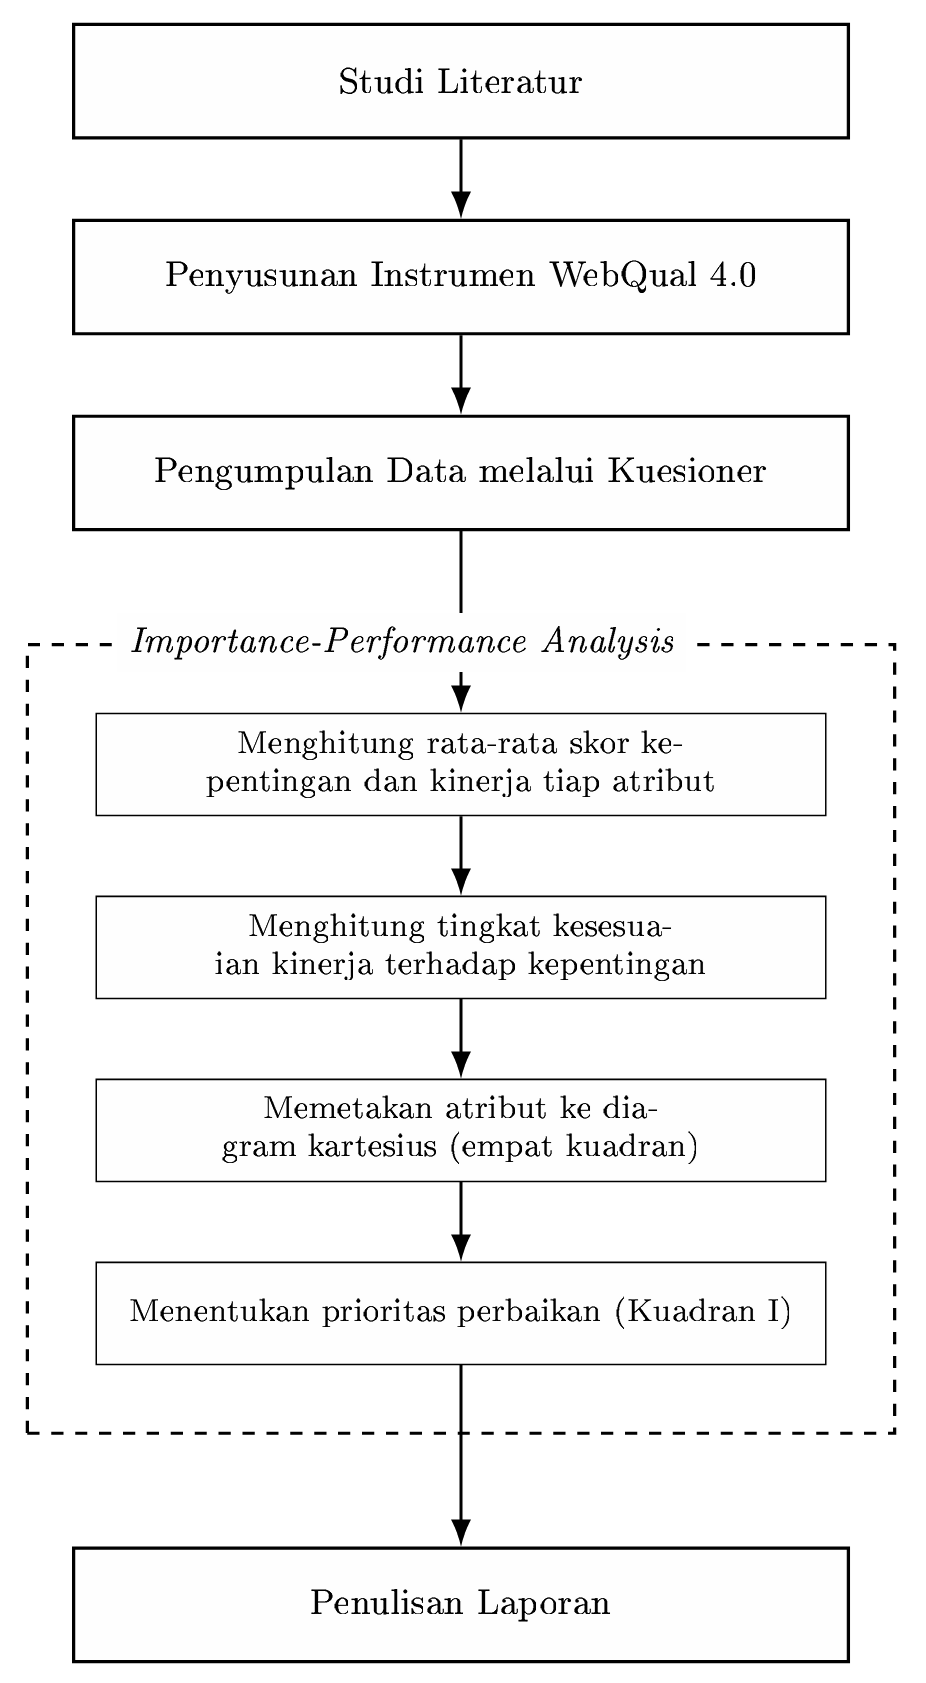
\includegraphics[height=7cm]{metode}   
    \caption{Langkah Penelitian}
    \label{fig:alurproposal}
\end{figure}

\subsection{Studi Literatur}
Pada tahap ini, dilakukan penelaahan mendalam terhadap literatur ilmiah terkini yang mendasari konsep antarmuka diegetik dan penanganan latensi. Literatur utama berfokus pada \textit{Diegetic User Interface} dan kaitannya dengan \textit{Player Immersion} serta \textit{User Experience}, rekayasa \textit{Asynchronous State Machine} pada \textit{game engine} untuk memisahkan eksekusi animasi fisik karakter dari \textit{background thread}, serta pengukuran \textit{Perceived Latency} dan \textit{Player Experience} (PX).

\subsection{Perancangan Prototipe Game 2D dan Skenario A/B Testing}
Pengembangan prototipe dirancang 2D dengan latar berada di Kampus Unika Atma Jaya BSD. Untuk menguji efektivitas penyamaran latensi, dibuat dua skenario perlakuan (\textit{treatment groups}) dengan durasi jeda waktu komputasi AI yang disimulasikan menggunakan fungsi pengacakan waktu (\textit{randomized delay/randint}) pada rentang X detik:
\begin{itemize}
    \item \textbf{Skenario A (\textit{Baseline / Non-Diegetic Group})}: Pemain mengajukan pertanyaan teks, lalu NPC Pustakawan berada dalam kondisi diam (\textit{idle/frozen}). Layar menampilkan komponen \textit{Non-Diegetic} UI berupa \textit{Loading Bar} atau teks "\textit{Thinking...}" selama X detik sebelum jawaban teks NPC muncul.
    \item \textbf{Skenario B (Eksperimen / \textit{Diegetic Latency Masking Group})}: Pemain mengajukan pertanyaan teks, lalu NPC memicu skrip animasi fisik kontekstual secara \textit{asynchronous} (misal: berjalan menuju rak buku atau memeriksa berkas dokumen) selama X detik yang persis sama, lalu NPC kembali ke meja dan jawaban teks muncul.
\end{itemize}

\subsection{Penyusunan Instrumen Evaluasi}
Instrumen penelitian disusun menggunakan kuesioner tertutup berskala Likert lima poin, sebagaimana disajikan pada \cref{tab:likertproposal}. Butir kuesioner dirancang untuk mengukur tiga variabel utama: \textit{Perceived Latency} (mengukur persepsi wajar/tidaknya waktu tunggu), \textit{Player Immersion} (mengukur penjagaan kontinuitas cerita fiksi \textit{game}), dan \textit{Player Retention \& Experience} (mengukur kenyamanan dan keinginan melanjutkan permainan).

\subsection{Populasi dan Sampel}
Populasi target penelitian ini adalah mahasiswa Teknik Aktif Universitas Katolik Atma Jaya BSD. Teknik pengambilan sampel menggunakan \textit{Convenience Sampling} dengan catatan bahwa mereka bersedia mengikuti prosedur \textit{playtesting} dua skenario interaksi secara utuh. Ukuran sampel ditetapkan sebanyak ~30 responden.

\subsection{Pengumpulan Data (Prosedur Playtesting)}
Pengumpulan data dilaksanakan melalui sesi \textit{user playtesting} langsung dengan protokol \textit{Within-Subjects Design} di mana setiap responden mencoba kedua skenario secara bergantian dengan urutan acak (\textit{counterbalancing}) untuk menghindari \textit{order bias}. Setelah menyelesaikan kedua skenario, responden mengisi kuesioner secara mandiri.

\begin{table}[H]
    \centering
    \caption{Skala Likert yang akan digunakan}
    \label{tab:likertproposal}
    \small
    \begin{tabular}{|c|l|}
        \hline
        \textbf{Skor} & \textbf{Pernyataan} \\ \hline
        1 & Sangat Tidak Setuju (STS) \\ \hline
        2 & Tidak Setuju (TS)         \\ \hline
        3 & Netral (N)                \\ \hline
        4 & Setuju (S)                \\ \hline
        5 & Sangat Setuju (SS)        \\ \hline
    \end{tabular}
\end{table}

\subsection{Teknik Analisis Data}
Data yang terkumpul dianalisis melalui dua tahap. Pertama, \textbf{Analisis Deskriptif} untuk menghitung nilai rata-rata (\textit{mean}), standar deviasi, dan median dari skor ketiga variabel utama. Kedua, \textbf{Uji Komparatif Statistik (Uji Beda)} untuk menguji signifikansi perbedaan antara Skenario A dan Skenario B. Uji ini diawali dengan Uji Normalitas (Shapiro-Wilk) dan dilanjutkan dengan \textit{Paired Sample t-Test} (jika normal) atau \textit{Wilcoxon Signed-Rank Test} (jika tidak normal). 
%dengan tingkat signifikansi $\alpha=0,05$.

\subsection{Penulisan Laporan}
Tahap akhir adalah penyusunan laporan yang merangkum seluruh proses dan hasil
penelitian menjadi naskah Tugas Akhir yang utuh.

\section{Matriks Keterkaitan Penelitian}
Agar penelitian tetap terarah, setiap rumusan masalah dipetakan terhadap data dan teknik analisis yang direncanakan, sebagaimana ditunjukkan pada \cref{tab:linkageproposal}.

\begin{table}[H]
    \centering
    \caption{Rencana keterkaitan penelitian}
    \label{tab:linkageproposal}
    \small
    \begin{tabularx}{\linewidth}{|c|X|X|}
        \hline
        \textbf{RQ} & \textbf{Data yang direncanakan} & \textbf{Teknik analisis} \\ \hline
        \cref{rq:design}    & Spesifikasi \textit{Asynchronous State Machine} \& \textit{Asset} animasi 2D NPC & Perancangan Sistem (\textit{Prototypes Engineering}) \\ \hline
        \cref{rq:evaluation} & Skor kuesioner \textit{Perceived Latency}, \textit{Player Immersion}, dan \textit{Player Retention} & Analisis Deskriptif dan Uji Beda Statistik \\ \hline
    \end{tabularx}
\end{table}

\section{Rencana dan Jadwal Penelitian}
Rencana pelaksanaan penelitian disusun selama enam bulan sebagaimana ditunjukkan pada \cref{tab:jadwal}. Sel yang diarsir menandakan bulan pelaksanaan tiap kegiatan.

\definecolor{jadwalisi}{gray}{0.25}
\begin{table}[H]
    \centering
    \caption{Rencana dan jadwal penelitian}
    \label{tab:jadwal}
    \small
    \begin{tabular}{|c|l|*{6}{>{\centering\arraybackslash}p{0.6cm}|}}
        \hline
        \multirow{2}{*}{\textbf{No.}} & \multirow{2}{*}{\textbf{Kegiatan}}
          & \multicolumn{6}{c|}{\textbf{Bulan}} \\ \cline{3-8}
         & & 1 & 2 & 3 & 4 & 5 & 6 \\ \hline
        1. & Studi Literatur \& Penyusunan Instrumen & \cellcolor{jadwalisi} & \cellcolor{jadwalisi} &                       &                       &                       &                       \\ \hline
        2. & Perancangan \& Pembuatan Aset Animasi 2D &                       & \cellcolor{jadwalisi} & \cellcolor{jadwalisi} &                       &                       &                       \\ \hline
        3. & Implementasi Prototipe Skenario A \& B  &                       &                       & \cellcolor{jadwalisi} & \cellcolor{jadwalisi} &                       &                       \\ \hline
        4. & Sesi \textit{Playtesting} \& Pengumpulan Data &                       &                       &                       & \cellcolor{jadwalisi} &                       &                       \\ \hline
        5. & Analisis Data Statistik \& Uji Beda     &                       &                       &                       &                       & \cellcolor{jadwalisi} &                       \\ \hline
        6. & Penyusunan Laporan Akhir \& Sidang TA   &                       &                       &                       &                       & \cellcolor{jadwalisi} & \cellcolor{jadwalisi} \\ \hline
    \end{tabular}
\end{table}        % BAB 3 RANCANGAN PENELITIAN (khusus proposal)

%------------------ BAGIAN AKHIR ----------------------------------
%==================================================================
% DAFTAR PUSTAKA  (dihasilkan otomatis dari a7-pustaka.bib)
%
% Hanya rujukan yang benar-benar disitasi di dalam naskah yang akan
% muncul di sini. Jika ingin menampilkan SELURUH entri pada berkas
% .bib meskipun tidak disitasi, aktifkan baris \nocite{*} di bawah.
%==================================================================
\clearpage
\phantomsection
\addcontentsline{toc}{chapter}{\bibname}
\begin{center}
    \textbf{\large \bibname}\\[1.5em]
\end{center}

% \nocite{*}
\bibliography{a7-pustaka}


\end{document}
